\documentclass[a4paper,12pt]{article}
\usepackage[T2A]{fontenc}
\usepackage[bulgarian]{babel}
\usepackage[utf8]{inputenc}
\usepackage{mathtools}
\usepackage{graphicx}
\usepackage{listings}
\usepackage{url}
\usepackage[pdfborder={0 0 0}]{hyperref}
\begin{document}
  \title{Създаване на Web-базирана система за подготовка на ученици за състезания по информатика}
  \author{Валентин Михов}
  \date{Август 2010}
  
  \maketitle
  
  \begin{abstract}
    
    В настоящата дипломна работа ще опиша опита ми в създаването на Web система за обучение на ученици по информатика. Ще опиша как за кратко време успях да изградя ядрото на системата, за имплементацията на което обикновенно отнема много време, като така успях да се концентрирам върху важните части на системата, които се ползват от учениците и ръководителите. Освен това ще споделя опита, който натрупахме заедно с още няколко колеги, докато използвахме тази система. Какво направихме добре и какво видяхме, че не работи при подготовката на състезатели по информатика.
  \end{abstract}
  
  \newpage

  \tableofcontents
  
 \newpage
  
  \section{Въведение}
    Това не е първата или последната разработка на автомаизирана система за оценка на задачи по информатика. Има много разработки по темата и не малко сайтове, които предлагат изключително добре направени системи, със изключително голямо количество задачи в тях. Така например Sphere Online Judge съдържа над 5000 задачи и 40 различни езика за програмиране \cite{online_judge_list}. Въпросът е защо решихме да направим още една такава и кому това е нужно? В тази глава ще разкажа, какво всъщност е състезателна система и как възникна идеята за Maycamp.
    
    \subsection{Състезателните системи.} Подробно описание на състезателните системи (СС) - предназначение, архитектура, основни функции и т.н., може да бъде намерено в \cite{grading_sys_manev}, затова тук ще се спрем съвсем накратко на техните характеристики. Всяка СС (на английски Grading system или прсто Grader), по своята същност представлява софтуерна система, която предоставя на участниците в състезания по програмиране възможност да изпращат решенията на състезателните задачи (изходен код на програма, написан на един от езиците за програмиране поддържани от системата). Системата архивира изпратеното решение, компилира го до изпълним код и проверява дали получената програма решава поставената задача, като изпълнява програмата върху зададено множество от тестове, в рамките на поставени ограничения за време и памет, и сравнява получените резултати с очакваните. 

    Това разбира се е доста опростено описание на същността на СС, тъй като в повечето случай една СС трябва да предоставя възможност за организиране на състезания по програмиране, за съхранение и визуализиране на условията на задачите, за генериране на класиране, поддръжка на различни видове задачи и оценявания и т.н. СС са изключително полезни при организирането на състезания по програмиране, тъй като автоматизират напълно тестването на решенията. Без използването на СС, тестването на програмите на състезателите се извършваше ръчно и отнемаше много време. Освен това СС може да автоматизира и други дейности, като генериране на класирания, статистики и архиви на състезанията. Една от първите състезателни системи е системата $PC^2$, днес официална състезателна система на ACM ICPC -- Международната олимпиада по програмиране за студенти \cite{pc2_home}. От 2000 година Международните олимпиади по информатика за ученици също използват състезателни системи, създавани обикновено от страната домакин. В организираните в България състезания по програмиране -- както национални, така и международни -- се използват системите SMOC \cite{smoc_system} и spoj0 \cite{spoj0_train}. 
 
    Практиката отдавна е показала, че СС са незаменим помощник за организаторите на състезания по програмиране. Интересното е, че не е толкова очевидно как една такава система може да помогне в обучението на ученици и студенти по програмиране. Има примери на СС, които се използват в процеса на обучение по програмиране. В \cite{intro_ribeiro} авторите описват опита си в прилагане на СС в обучението по програмиране в Португалия. Системата spoj0 се използва активно във Факултета по математика и информатика на Софийския университет при преподаване на курсове по алгоритми. Елементи на обучение предлага, например, системата USACO за подготовка на американските ученици, които се готвят за участие в Международната олимпиада по програмиране \cite{usaco_training}. 
 
    За съжаление, споменатите системи не са много популярни сред учениците в България, особено сред по-малките. Това се дължи до голяма степен на факта, че тези системи са ``затворени'' в рамките на съответните институции или за използването им е необходимо добро владеене на чужд език (най-често английски), което прави използването им от по-малки ученици трудно или невъзможно. 
 
    Разглежданият в тази статия проект има за цел да подпомогне подготовката на начинаещи програмисти с използване на състезателна система. В раздел 2 е представена една ранна фаза на проекта и някои негови недостатъци. В раздел 3 са формулирани проектните идеи, които трябваше да ни приближат по близко да целта на проекта. В раздел 4 са представени някои резултати от едногодишната работа на сайта, а в раздел 5 - насоки за бъдещи усъвършенствания.
    
  \subsection{Идеята за Maycamp}
  
  Нека първо да разясния кой сме ние и как започна всичко. Всичко започна в един обед в София, когато бяхме заедно със моя колега Слави Маринов в един ресторант. Разговаряхме за това как образованието в България е доста счупено и има нужда от нещо, което да го оправи. Слави имаше идеята да направим промяна в подготовката по информатика: нещо в което имаме познания и опит. Останалото ще дойде с времето. Това беше началото. Една проста идея: да подобрим подготовката по информатика в България.
  
  След известно време вече бяхме събрали доста съмишленици, най-вече сред бившите състезатели по информатика, които са останали в България. Събрахме се не малко хора: Антон Димитров, Тодор Петров, Орлин Тенчев, Слави Маринов, Даниел Славов, Кремена Роячка, Слави Маринов, Пламена Александрова и аз.
  
  Първоначалната идея беше да се направи сайт, на който да се публикуват видео лекции. Лекциите са организирани на нива и за да можеш да преминеш на следващото ниво трябва да решиш задачите от текущата лекция, като така показваш, че си разбрал материала. Освен това всеки участник има ментор, който му помага когато има трудности.
  
  След едногодишна работа се оказа, че този формат не е толкова ефективен, колкото на нас ни се иска и е труден за поддръжка от хора, които се занимават само през свободното си време с това. Всички хора в проекта работихме на пълен работен ден и трябваше да вместваме работата по проекта в графика си. Така на годишната сбирка на екипа, след като разгледахме резултатите от анкетата, която проведохме сред учаснитиците, решихме да сменим формата на подготовката. Почти всички участници бяха посочили, че ако правим тренировъчни състезания това ще подобри новото им много повече. Така решихме да направим система, на която да даваме състезания.
  
  Системата не беше единственото нещо, което решихме да създадем. Освен редовните състезания и възможността за практика на стари задачи, решихме на сайта да има и анализи на решенията, както и статии на различни теми, като например стратегии за решаване на задачи на състезание.
  
  Беше решено, че ще направим 12 състезания през годината, като всяко състезание ще има 3 дивизии: бронзова, сребърна и златна, като разликата ще е в нивото на трудност. Идея, която взаимствахме от USACO \cite{usaco_website}. След всяко състезание ще се публикуват анализи на задачите и всяка задача ще може да се практикува, като ще има класация по практика. Освен това задачите ще се оценяват на принципа на ученическите състезания, като на една задача можеш да имаш между 0 и 100 точки според това за какъв процент от тестовете програмата ти работи.
  
  \subsubsection{Защо още една система}
  
  Един от най-важните въпроси и е защо решихме да правим изцяло нова система, след като има толкова много готови. Разбира се ние мислихме по този въпрос и като крайно прагматични хора разгледахме алтернативите. Ето и причините, които ни накараха да поемем по този път:
  
  \begin{enumerate}
    \item Искахме всички материали да са на български език - след като направихме проучване сред състезателите, се оказа че по-малките сстезатели имат проблем с подготовката от сайтове на английски език. Тъй като според нас малките състезатели са много важни (дори може би по-важни от големите), решихме че това е много важен аргумент, който трябва да имем предвид.
    \item Искаме задачите да се оценяват на принципа на ученическите състезания. Оказва се че повечето системи за подготовка се основават на ACM правилата, които гласят че една задача е или решена за 100 точки или не е решена, т.е. 0 точки. Това не беше допустимо за нас, тъй като на едно ученическо състезание е от много голямо значение всеки състезател да може да извлече всяка една точка. Това, че не може да измисли решението за 100 точки не значи, че трябва да се откаже от дадена задача. Това според нас е умение, което трябва да се тренира в участниците.
    \item Искаме да даваме лесни задачи в бронзовата дивизия. Спред нас това е жизнено важно за привличането на нови състезатели в малките възрастови групи. Повечето системи за подготовка наблягат на сериозните състезания, което кара малките и нови състезатели да се отчайват от трудността на задачите. Нашата цел е точно обратна - да накраме тези по-малки и неопитни деца да усетят тръпката на състезанието и победата над съучениците им.
    \item Възможността ние да контролираме всеки един аспект от системата. Свободата, която ще имаме ако системата е наша е много важна за да можем да вървим напред. Разбира се това идва на цена: повече време отделено за разработка и нуждата да поддържаме сами всичко.
  \end{enumerate}
  
  Разбира се ние сме наясно, че няма вечни неща на този свят и е възможно в близко бъдеще да се появи нова система правена от други хора, която да засенчи нашата. Затова и целта беше да изградим това начинание с възможно най-малко усилия, без да се задълбаваме в техничеки подробности. В следващите глави ще опиша какви решения направихме по време на имеплементацията и как всъщност с доста малко усилия изградихме всичко.
  
  \section{Изграждане на системата}
  В следващата секция ще проследя етапите през, които премина изграждането на
  Арената. Ще се опитам да опиша какво беше направено добре и какво не.
  \subsection{Изграждане на ядрото за пускане на код}
  Във всяка една система за провеждане на систезания по програмиране има ядро,
  което се занимава със пускане на решенията на участниците в контролирана среда
  и оценка на решенията срещу дадено множестно от тестове.

  Обикновенно ядрото на системата включва в себе си модул, който умее да пуска код в контролирана среда - така нареченият sandbox. Идеята на този модул, е че кода който състезателите пращат обикновенно не е коректен и пускането му може да доведе до нестабилност във системата. Освен това е нужен за да се продотврати опити за хакване на системата или за измами, като се пращат решения, които по заобиколен и нечестен начин успяват да работят за 100 точки.
  
  Има много публикации за това как може да бъде направен един подобен модул. Това е доста сложна тема и един такъв модул може да е изключително сложен. Може би това е най-трудната част в имплементирането на една подобна система.
  
  Единият от начините е да се направи модул към ядрото на Linux, с който да се следи какво прави изпълняваният код. За повече информация можете да видите \cite{linux_sec_module_sandbox}, където е анализирано подобно решение. Оказва се обаче, че подобна имплементация има доста проблеми, като например често сменящи се интерфейси за модулите за сигурност на Linux, не добра документация и като цяло не добра поддръжка на този вид модули от екипа разработващ ядрото на Linux. Освен това е добре да се отбележи, че подобен модул няма да е никак тривиален за имплементация, тъй като изисква дълбоки познания за ядрото в Linux и работа с недокументирани интерфейси.
  
  Другият начин за справяне с този проблем е с прихващане на системните извиквания. Подобно решение е ползвано и в системата Moe и повече за него може да бъде прочетено тук \cite{perspectives_grading_systems}. Накратко идеята е да се ползва така нареченият ptrace интерфейс в Linux, с който кода на състезателя за пуска в контролирана среда и всяко едно системно извикване от кода се прихваща и проверява от контролиращият модул. Ако контролираният код направи системно извикване, което не е позволено, то той се прекратява и се смята, че участника се опитва да направи нещо против правилата.
  
  Това е може би най-широко използваният в момента модел, като ситемите на IOI използват точно него. За нещастие и той има някой слаби страни: може да забави доста тестването на решенията \cite{performance_reactive_tasks}, а и не е никак тривиален за имплементация.
  
  Трябва да се отбележи, че подобни модули вече съществуват и дори могат да се ползват на готово, както например беше направено на международната олимпиада в България 2009 \cite{validating_security}. Модулът, който се ползва на тази олимпиада е от системата Moe и вече е ползван на няколко големи олимпиади и показва стабилни резултати. За съжаление, когато аз започнах да разработват системата за Maycamp, не знаех за съществуването на този модул, а нямах никакво време за да имплементирам сложни решения. Така стигнах до решение, което е доста просто като логика, много кратко и след 11000 тествани решения и над 10 проведени състезания е показало незначителни проблеми, за които ще напиша по-нататък.
  
  Решението, което предлагам предоставя защити срещу няколко основни типове атаки и мисля, че до голяма степен елиминира 95\% от възможните хакове, които биха могли да бъдат пробвани.
  
  \subsubsection{Импементация на модула за контролирано пускане на код}
  Когато започнах изграждането на модула, първото нещо което направих беше да идентифицирам основните ситуации, които искам модулът да засича. Това са:
  
  \begin{enumerate}
    \item Решения, които зациклят в безкраен цикъл
    \item Решения, които заспиват в системно извикване (например getc())
    \item Решения, които се опитват да заделят повече памет от позволеното
    \item Безкрайна рекурсия
    \item Fork-бомба
    \item Опити за установяване на мрежова връзка
  \end{enumerate}
  
  Въз основа на тези основни проблеми, направих проста система за тестване, която симулираше всяка от тези ситуации и проверяваше дали изграденият модул се справяше с тях. Самият модул представява скрипт, който приема като аргументи параметрите, в които решението трябва да се изпълни и като прикючи, в статуса му има код, който описва дали това се е случило. Ако по време на изпълнението е визникнала извънредна ситуация, статусът описва какво точно е станало. Ето и псевдо-код на скрипта:
  
  \begin{lstlisting}
    fork the current process
    in the child:
      set limit of the number of child processes
      set the priority of the current process to the lowest
      
      execute the program to be tested
    
    in the parent:
      while the child process is running:
       check the running time of the child process
       check the used memory of the child process
       check the running state of the child process
       
       if any of these are out of expected, kill the process
       
      process the exit status of the child process
  \end{lstlisting}
  
  Както виждате първото нещо, което прави той е да клонира текущият процес и да заложи накой от параметрите на новият процес. Задаването на брой позволени процеси става посредством setrlimit. След проведени тестове се оказа, че това работи стабилно под Linux и предотвратява атаките със fork-бомби, които са може би едни от най-лесните и най-опасните за подобна система.
  
  След това се сваля приоритета на новият процес до минимума, като така се гарантира, че нашият скрипт, които ще следи решението ще се изпълнява достатъчно често за да може своевременно да засече всякакви нередности.
  
  Накрая новият процес пуска кода на програмата за тестване, която напълно заменя новият процес.
  
  През това време в процеса-баща вървят постоянни проверки за състоянито на процеса-дете. На много малки интервали от време се проверява във proc файловата система, колко точно време и памет е използвана, както и състоянието на самият процес. Ако по време на една такава проверка се види, че процесът е заспал, то значи той прави нещо нередно. Нито едно от системните извиквания, които са позволени на състезателите не могат да накарат програмата да е в състояние sleep. Това означава, че е направено системно извикване, което чака някакви данни да се получат или за някакво друго събитие. Задачите, които се тестват на тази система, винаги четат от стандартният вход и пишат на него и това са едиствените системни операции, които им са позволени. Освен това винаги когато едно такова решение бива извикано, входните данни са подадени на стандартният вход, т.е. не се очаква решението да заспи в чакане на входни данни.
  
  Така чрез тези няколко изключително прости механизми се гарантира прихващането на изброените по-горе сценарии.
  
  % ********************************* Архитектура ******************************
  \subsection{Архитектура на системата}
  При изграждането на Арената, реших че е крайно неприемливо цялата система да е
  на една физическа машина. Тъй като пускането на чужд код е една крайно несигурна операция, дори и в конролирана среда, възможността при евентуална атака цялата система да бъде компрометирана ми се струваше крайно неприемлива. Затова и решението беше решенията да се оценяват на машина, която е изцяло независима от системата, която поддържа Web интерфейса към системата. Така ако има атака, чрез пращане на опасен код, сайта ще продължи да работи, а машината, която тества ще бъде афектирана - Фигура~\ref{architecture}.
  
  \begin{figure}
    \begin{center}
      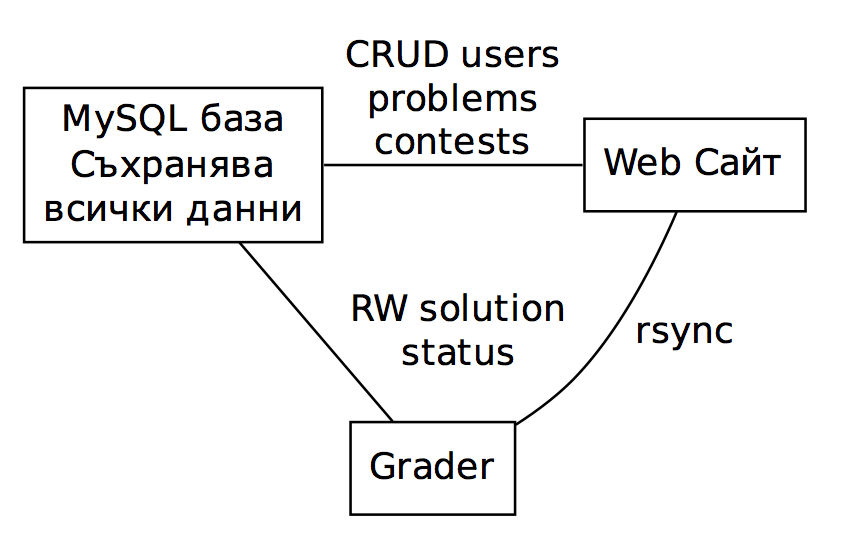
\includegraphics[width=0.8\textwidth]{architecture.png}
    \end{center}
    \caption{Архитектура на системата}
    \label{architecture}
  \end{figure}
  
  Това е доста прост начин за изолация и не е никак нов при изграждането на подобни системи. Тъй като при нас все още данните са сравнително малко решихме да обединим MySQL машината с Web машината, като така намалим разходите си за инфраструктура. Така цялата система се състои от 2 машини. Едната се хоства в dreamhost.com, сериозен доставчик на подобни услуги, а другата се намира в България, на сървър, които ние закупихме за разнообразни нужди. Така израдената архитектура има своите определени преимущества, но има и някой недостатъци, с които трябваше да се преборим.
  
  Първият проблем, е скоростта на комуникация между отделните машини. В нашият случай Web частта се намира на чуждестранни сървъри, където сме сигурни, че машината ще работи 99\% от времето и ще е свързана постоянно към Интернет. От друга страна машината, която оценява решенията се намира в България. За всяко едно оценяване на решение трябва да се осъществи комуникация между двете машини, като скороста между тях е многократно по-малка от скоростта ако те бяха в една локална мрежа. Това прави нужно да се минимизира комуникацията между тях. Затова решихме двете машина да обенят единствено сорс кодовете на решенията, резултатите от тестването и логовете от тестването на решението.
  
  Това решение се оказа добро, но малко след пускането на системата се оказа, че има проблем в него. Проблема, беше не толкова в архитектурата, колкото в конкретната имплементация. Оказа се, че ако някое решение генерира много голям вход, лога на тестването става много голям, тъй като той съдържа разликата между правилният отговор и отговора на състезателя. Така ако разликата е много голяма комуникацията между Web частта и Grader-а се задръства. Това наложи да сложим ограничения на размера на показваната разлика в лога, което реши проблема.
  
  Вторият проблем е как да се пазят тестовете на задачите. Те могат да са доста големи и както видяхме в предната точка не е приемливо много данни да се прехвълят при всяко тестване. Така решихме да пазим две копия на тестовете. Едно на Web сървъра и едно на тестващият сървър. Въпросът е как синхронзираме тези две копия?
  
  Първо за да можем да сме сигурни, че във всеки един момент тестваме с най-новите тестове, преди всяко тестване се проверява поле в базата, което пази последната дата на промяна на тестовете. Ако тази дата е по-нова от датата на тестовете, които има на Grader-а в момента, тестовете се обновяват. За да работи тази схема коректное е нужно двата сървъра да имат синхронизирано време. За целата за използва NTP улугата, която синхронизира часовниците на сървърите с точното време взето от световни сървъри предназначени за това.
  
  Първоначално бях направил синхрониацията да става с изтегляне на zip файл със тестовете, но това доста бързо се оказа неподходящо. В момента тестовете на всички задачи заемат 945Mb некомпресирани, но дори и компресирани това е доста голямо количество данни за пренос между двата сървъра. За целата направих решение използващо rsync, което копира единствено променените файлове между двата сървъра. Това се оказа прекрасно решение! Авторите на задачи могат в рамките на секунди да качат нова задача и да я тестват. Времето за синхронизация на тестовете е на практика незабележима.
  
  \subsection{Изграждане потребителският интерфейс}
    Една от основните цели, които си поставихме при създаването на състемата, беше потребителският интерфейс да е лесен за ползване и да имаме възможност да о променяме по лесен начин. Тъй като аз бях човека, който основно разработваше кода, реших да ползваме за изграждането на системата Ruby on Rails \cite{rubyonrails_site}. Това мое решение беше продиктувано от опита ми с тази библиотека и увереноста, че тя ще ни предостави лесен начин за разработване на потребителският интерфейст, както и лесен начин за неговата промяна с времето. Всъщност една от силните страни на Ruby on Rails е неговата гъвкавост и липса на "поддържащ код", т.е. код, който не е свързан пряко със основната функционалност на системата.
    
    По време на разработката на потребителският интерфейс се придържахме към итеративен процес. Аз разработвах парче нова функционалност и след това няколко човека започвахме да го ползваме. В процеса на ползване се откриваха проблеми и недостатъци, които се оправяха. Създаваха се и интеграционни тестове, които спомагаха да се откриват регресии своевременно. За разработване на тестовете се ползваше cucumber \cite{cucumber_site}. Това е библиотека за тестване на високо ниво, като в общи линии тестовете симулират човешки действия на сайта, като например: отваряне на дадена страница, следване на линк от текущата страница, попълване на форми и пращенето им и други. Тестването е много съществен елемент в едно подобно гъвкаво разработване на система, тъй като нещата се променят много бързо и е много лесно части от системата да спрат да работят. Подържането на добро множество от тестове, които освен това се пускат автоматично след всяка качена промяна на кода е ключово за това процеса на работа да върви безпрепятствано.
    
    Последният елемент, който допълнително направи разработката много гъвкава беше разработването на система за обновяване на сайта с едно кликване. Това означава, че след като някаква промяна е направена и качена в централното хранилище на кода, за няколко минути се вижда дали няма регресии (функционалност, която е спряла да работи) и след това само с една команда и в рамките на секунди новият код може да се качи на сайта и да бъде достъпен за всички потребители. За разработването на това автоматизирано обновяване ползвахме capistrano \cite{capistrano_site}.
    
    Този процес ни осигури много голяма гъвкавост и изключително кратко време на реакция при откриване на проблеми или нуждата за разработване на нова функционалност. Тези основни елементи са нещо, което мога да пропоръчам при разработването на всеки един проект. Възможността да във всеки един момент да се види каква е текущата версия и да може да се качи обновена верися в рамките на секунди са незаменими възможности при разработката на един софтуер.
  \subsection{Формат на състезанията и задачите}                              
    Формата на състезанията и задачите и много подобен на този на системата spoj0. Това е така, тъй като в началото системата Arena започна като разклонение на spoj0. В последствие кода толкова много се промени, че в момента двете системи почти нямат нищо общо, но формата остана същият, което е добре, тъй като позволява много лесно състезания да се качват от spoj0 на Arena.
    
    Най-общо едно състезание има две части: част която се пази в база данни и част, която се пази на файловата система. На практика всичко освен условието на задачата, тестовете и чекъра се пазят в базата. Това са името на задачите, ограниченията за време и памет, продължителността на състезанието и решенията на участниците. Както може да се забележи това е най-вече мета информация за състезанието, която е нужно да бъде лесно и бързо достъпна за да работи сайта добре. Информацията, която се пази на файловате система се ползва най-вече от \"grader\"-а, който оценява решенията. Това е защото се предполага, че grader-а може да е отдалечена машина и неговият достъп до базата данни е по-бавна. Това прази невъзможно да се пазят големи данни в базата, тъй като биха забавили много оценяването.
    
    Както споменахме по-рано тестовете на задачите са доста голям обем от информация, достигат почти 1ГБ и се увеличават стремително. Интересен е проблема как тези данни се дистрибутират на машините, които оценяват решения. Отговова е много прост: rsync \cite{rsync_site}. Това е инструмент с отворен код, който се ползва широко за синхронизация на масиви от данни между няколко машини. Хубавото на този инструмент, е че пренася само променените файлове, т.е. ако се качат тестове на нова задача, единствено тези нови тестове се синхронизират между системите, които оценяват. Така след като се качи ново състезание в рамките на секунди grader-ите получват новите тестове на състезанието и са готови да тестват решения. Аналогично ако тестовете се обновят или дадено състезание се изтрие, отново в рамките на секунди промените се пренасят на всички машини.
    
    TODO: describe the format of the checkers, the description and input/output files.
  \subsection{Описание на системата за рейтинги}
  
  
  \subsubsection{Математически модел}
  В тази секция ще разясня как точно работи модела на рейтингите на арената. Както вече казах, решихме да използваме системата за рейтинги на TopCoder \cite{topcoder_ratings}. Въпреки, че математическият модел е описан като формули на сайта на TopCoder, каква е идеята зад самият модел не е толкова очевидно.

  В тази секция ще се опитам да разясня как работи този модел, а в следващата секция ще видим защо всъщност е добър за нашите цели.
  
  Модела е статистически и приема, че при едно състезание разпределението на точките е нормално. Това значи, че хората с най-малко точки са малко, после тези със около среден брой точки най-много и тези които са с най-много точки също са малко. Виж Фигура~\ref{normal_distribution} за нагледен пример.
  
  \begin{figure}
    \begin{center}
      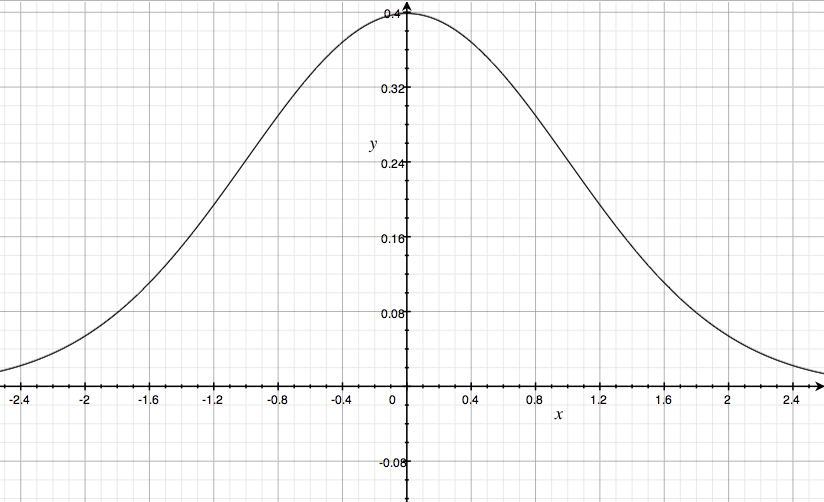
\includegraphics[width=0.8\textwidth]{normal_distribution.png}
    \end{center}
    \caption{Нормално разпределение}
    \label{normal_distribution}
  \end{figure}
  
  Системата за оценяване пази 2 стойности за всеки състезател: текущ рейтинг и променливост. Рейтинга е оценка на състезателя спрямо останалите състезатели, а променливостта оценява до колко представянията на този учасник са постоянни, т.е. ако състезателя винаги е на първо място неговата променливост ще е малка, но ако понякога е на първо и понякога на последно място, тогава променливостта му ще е голяма. Можем да си мислим и за рейтингите като случайни величини, а променливостта е тяхната дисперсия. 
  
  След всяко състезание, алгоритъма преизчислява рейтингите и променливостта. Алгоритъма, който прави това взема като вход класиране на състезатели, техните рейтинги и тяхната променливост. Трябва да се отбележи, че това колко точки има всеки състезател е без значение. Важно е единствено мястото в класирането. Ако двмата състезателя имат равен брой точки, то се смята че те са на едно и също място, което е средното аритметично от местата покрити от тях, т.е. ако има трима човека на 1 място с равен брой точки, т.е. те са все едно на \((1 + 2 + 3) / 3 = 2\) място.
  
  Отначало се изчислява средният рейтинг на учасниците в състезанието:
  
  \begin{equation} \label{eq:ave_rating}
    AveRating = \frac{\sum\limits_{i=1}^{NumCoders} Rating_{i}}{NumCoders}
  \end{equation}
  
  Важно е да се отбележи, че винаги се съпоставят състезатели, които са участвали на едно и също състезание с едни и същи задачи.
  
  В тази формула \(Rating_i\) е рейтинга на \(i\)-тият състезател, а \(NumCoders\) е общият брой състезатели.
  
  Следващата стъпка е да че изчисли, конкурентността на състезанието. Това е число, което зависи от две компоненти. Първо от средното квадратично от променливостта на всички състезатели, и второ от това колко са различни рейтингите на всички състезатели. Колкото повече състеатели има със различни рейтинги, толкова това число е по-голямо. Ето и формулата която се ползва: 
  
  \begin{equation}
    CF = \sqrt{\\
      \frac{\sum\limits_{i=1}^{NumCoders}Volatility_i^2}{NumCoders}\\
      +\\
      \frac{\sum\limits_{i=1}^{NumCoders}(Rating_i-AveRating)^2}{NumCoders - 1}\\
    }
  \end{equation}
  
  Идеята е, че колкото по-конкурентно е едно състезание, толкова повече точки носи то.
  
  Следващата формула е може би една от най-интересните. Това което се опитва да изчисли тя е каква е вероятността един състезател да има повече точки от друг състезател, т.е. да е по-напред в класирането от него. Тъй като предполагаме, че разпределението е нормално, можем да използваме функцията за грешка на нормалното разпределение и да използваме разликата на рейтингите на двамата състезатели. Функцията за грешка има стойност 0 за 0, което ще рече, че ако имаме двама състезателя с еднакъв рейтинг то шанса всеки един от тях да е по-напред от другия е 0.5, т.е. те имат равни шансове. Както виждате на Фигура~\ref{error_function} тази функция има много подходяща графика, която е много стръмна около нулата и постепенно става по-полегата, т.е. колкото е по-голяма разликата в рейтингите на двамата състезателя, толкова преимущестовото на по-силният ще е по-малко осезаемо.
  
  \begin{figure}
    \begin{center}
      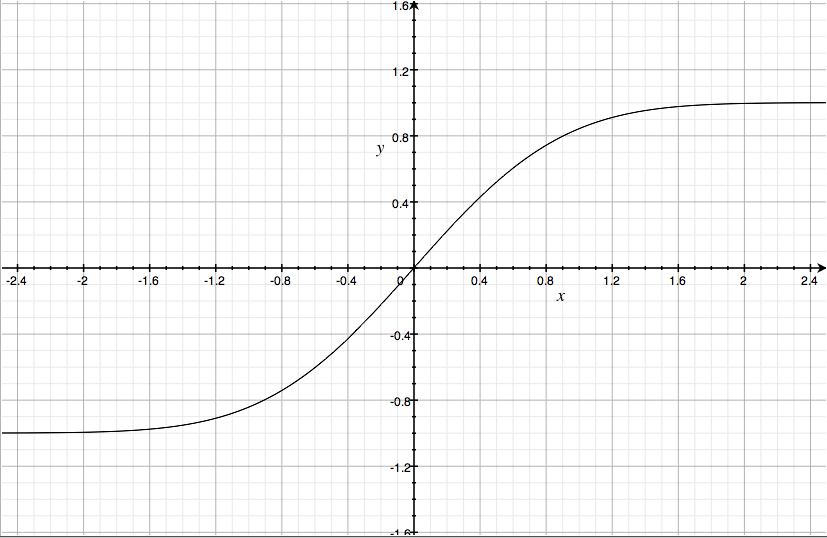
\includegraphics[width=0.8\textwidth]{error_function.png}
    \end{center}
    \caption{Функция на грешката}
    \label{error_function}
  \end{figure}
  
  Тъй като рейтингите, са на практика случайни величини и когато ги изваждаме ние създаваме нова случайна величина. Затова трябва да разделим разликата на тяхната комбинирана дисперсия. Освен това имаме условието при равни рейтинги вероятността да е 0.5, което ни води към следната формула:
  
  \begin{equation}
    WP=0.5\left(erf\left(\frac{Rating1 - Rating2}{\sqrt{2(Vol1^2+Vol2^2)}}\right) + 1\right)
  \end{equation}
  
  След като имаме тази формула, можем да изчислим вероятността всеки състезател да победи всеки друг и така можем да изчислилим предполагаемото място на всеки състезател в класирането:
  
  \begin{equation}
    ERank=0.5+\sum\limits_{i=1}^{NumCoders} WP_i
  \end{equation}
  
  Където \(WP_i\) е вероятността текущият състезател да победи състезателя с номер \(i\).
  
  Следващата стъпка е да изчислим каква е вероятността състезателя да е на оцененото място. Това е лесно тъй като предполагаме, че състезателите са разпределени нормално в класирането, така че ще ползваме обратната на комулативната функция на нормалното разпределение \(\Phi\). Тук изваждаме 0.5 и делем на брой състезатели, за да можем да работим с нормалното разпределение, което работи с интервала \((0..1)\).
  
  \begin{equation}
    EPerf=-\Phi\left(\frac{ERank - 0.5}{NumCoders}\right)
  \end{equation}
  
  По аналогичен начин изчисляваме реалното представяне на състезателя като вземаме неговото реално място \(ARank\) в състезанието и изчисляваме каква е вероятността той да е на него:

  \begin{equation}
    APerf=-\Phi\left(\frac{ARank - 0.5}{NumCoders}\right)
  \end{equation}
  
  Така можем да изчислим представянето на състезателя като рейтинг. Това е разликата между това което очакваме и това което реално той е показал умножено по конкурентността на състезанието плюс старият рейтинг на състезателя:
  
  \begin{equation}
    PerfAs = OldRating + CF*(APerf - EPerf)
  \end{equation}

  Тук е много важно да отбележим какво става, когато едни състезател участва за първи път. В този случай той няма реално рейтинг в системата и за целта му слагаме фиктивен такъв. Всеки нов състезател започва със рейтинг 1200 и променливост 515. Освен това в началото се позволява на състезателите да си променят по-бързо рейтинга и за целта че изчислява функция на тежестта, която зависи от броя участия на състезателя:
  
  \begin{equation}
    Weight = \frac{1}{1 - \left(\frac{0.42}{timesPlayed + 1} + 0.18\right)} - 1
  \end{equation}
  
  Освен това се изчислява и максимална промяна на рейтинга:
  
  \begin{equation}
    Cap = 150 + \frac{1500}{TimesPlayed + 2}
  \end{equation}
  
  Накрая се изчислява новият рейтинг по този начин:
  
  \begin{equation}
    NewRating = \frac{Rating + Weight * PerfAs}{1 + Weight}
  \end{equation}
  Като, ако \(|NewRating - Rating| > Cap\), то NewRating се намества така, че той да не се променя повече от \(Cap\).
  
  Освен това се изчислява и новата променливост, която е приближение на дисперсията на случайна величина, като се има предвид и тежестта на състезанието:
  
  \begin{equation}
    NewVolatility=\sqrt{\\
    \frac{(NewRating - OldRating)^2}{Weight}\\
    +\\
    \frac{OldVolatility^2}{Weight + 1}\\
    }
  \end{equation}
  
  \subsubsection{Примери}
  След като разяснихме как работи модела, нека да разгледаме малко примери за да видим защо всъщност този модел е успешен и как той ни помага.
  Нека например да разгледаме резултатите от състтезанието Арена 8 от 2010 година:
  {\tiny
    \begin{center}
      \begin{tabular}{ | l | l | l | l | l | l | l |}
        \hline
        Място & Oчаквано място & Участник & Точки & Стар рейтинг & Нов рейтинг & Разлика \\ \hline
        1 & 1 & Антон Анастасов & 195 & 2104.28 & 2165.4 & 61.12 \\
        2 & 6 & Momchil Peychev & 175 & 1548.29 & 1660.53 & 112.24 \\
        3 & 4 & Йордан Чапъров & 165 & 1654.95 & 1707.54 & 52.59 \\
        3 & 9 & Тодор Марков & 165 & 1358.14 & 1469.44 & 111.3 \\
        5 & 3 & Николай Хубанов & 135 & 1751.74 & 1736.54 & -15.2 \\
        5 & 7 & Dimitar Hristov Hristov & 135 & 1499.91 & 1538.06 & 38.15 \\
        7 & 10 & Михаил Ковачев & 130 & 1304.56 & 1344.68 & 40.12 \\
        8 & 11 & Красимир Георгиев & 105 & 1281.06 & 1294.7 & 13.64 \\
        9 & 5 & Никола Таушанов & 100 & 1611.43 & 1550.93 & -60.5 \\
        10 & 12 & Емануел & 55 & 1196.11 & 1189.25 & -6.86 \\
        11 & 13 & Александър Коджабашев & 35 & 1057.37 & 1048.67 & -8.7 \\
        12 & 8 & Михаил Карев & 25 & 1385.14 & 1308.65 & -76.49 \\
        13 & 2 & Румен Христов & 0 & 1996.16 & 1738.96 & -257.2 \\
        13 & 14 & Владимир Владимиров & 0 & 1011.67 & 952.8 & -58.87 \\
        13 & 15 & zelenkroki & 0 & 750.03 & 742.64 & -7.39 \\
        \hline
      \end{tabular}
    \end{center}
  }
  
  Участниците са наредени по това колко точки имат на състезанието, а в колоната "Очаквано място" е мястото, което се предполага те да заемат спрямо тяхният рейтинг. Това всъщност е критерият, който се ползва от системата за рейтинги.
  
  Както можете да видите Антон Анастасов е на 1 място, и това не неговото очаквано място. Затова и той си увеличава рейтинга, но не с много. От друга страна на второ място е Момчил Пейчев, който е успял да изпревари 4 състезателя с по-голям рейтинг от неговият, т.е. той се е представил много по-добре от колкото рейтинга му предполага и затова полуачава доста по-голямо увеличение на рейтинга. От друга страна ако разгледаме Румен Христов, той е със втори най-голям рейтинг, но се е класирал с 0 точки и респективно получава най-съществено намаляване на рейтинга.
  
  zelenkroki е с най-нисък рейтинг преди състезанието, класира се на последно място, т.е. това е напълно очаквано и както виждаме рейтинга на този състезател почти не се променя.
  
  Така както виждаме алгоритъма се опитва да "окуражи" състезателите да се представят по-добре от състезатели с по-голям рейтинг от техният, както и да наказва състезатели, които са с висок рейтинг, но постигат ниски резултати. Това е много подходяща схема за оценяване, тъй като взема предвид как се е представял един състезател преди състезанието и ако един състезател с много нисък рейтинг се представи добре на състезание от по-високо ниво, той ще напредне много бързо, докато ако състезател с много високо ниво участва на състезание, на което участват само състезатели с по-нисък рейтинг от неговият той няма да спечели много точки ако е на 1 място, докато ако не се представи добре ще загуби много точки. Тази система ни накара да мислим, че рейтинги ще накарат състезателите да участват в дивизии от техният ранг, както и, че ще имаме възможност въз основа на рейтингите да правим разграничаване на състезателите и да им позволяваме да участват в състезания от по-ниско ниво, ако преди това са показали че са много добри.
  
  \subsubsection{Прибавяне на външни състезания}
    След като интегрирахме системата за рейтинги се подори идеята да я използваме върху нацоналните състезания по програмиране. Ако можем да добавим тези състезания към алгоритъма ще можем да получим нещо като национална ранклиста на състезателите по програмиране и ще можем да следим как се движи нивото им (рейтинга) във времето. Това е много добра идея, но как ще свържем състезателите от националните състезания със потребители на арената?
    
    Подхода, който избрахме е да ползваме имената и града, от който са състезателите. Тъй като в арената имаме информация, от кой град е всеки потребител, то можем да филтрираме потребителите от даден град и да се опитаме да съвпаднем имената. Критерият, които използвахме е да гледаме за поне 2 съвпадения на имена, т.е. раделяме името на състезателя на отделни думи и гледаме за поне 2 съвпадащи думи. Освен това пазим история за това кое име с кой потребител сме свързали и ако пак срещнем това име от този град използваме същият потребител. Това ни дава възможност ръчно да свържем някой състезател с потребител от системата и да може след това автоматично да свързваме този състезател с правилният потребител.
    
    Интересно е и как осъществихме лесно въвеждане на резултатите от състезанията в системата. Тъй като много често резултатите се качват като Excel таблици в интернет, много лесно от таблиците може да се copy/paste-нат резултатите, които се появяват като таблица използваща табулации за разделители. Това позволява лесно да се обработят тези таблици и да се въведат в системата, след което алгоритъма за свързане на имена към потребители се пуска върху данните. За повече информация вижте екраните представени в секцията с описание на системата.
  \subsubsection{Национална ранклиста на състезателите}       
  Така логично се стигна до идеята да се направи национална ранклиста на състезателите по рейтинги. Класирането по рейтинги е много по-мощно средство от това просто да се сумират точките от състезанията, тъй като мястото е това което е опреелящо за един състезател и чрез неговият рейтинг много лесно могат да се изследват тенденции в представянето на състезателите. Много лесно може да се види, кой състезател се нмира в добра форма и напредва бързо, както и състезатели, които се представят под нивото си и изостават.
  
  За съжаление подържането на такава ранклиста изисква редовно качване на най-новите класирания от национални състезания, както и постоянно подобряване на алгоритъма за свързвне на имена със потребители от системата. За момента нямаме толкова много ресурси за да провеждаме това и едната такава ранклиста остава все още идея в процес на разработка.
  \section{Анализ на постигнатото до момента}
  \subsection{Статистика за посещаемостта на системата}
  \subsection{Анализ на анкетите пратени към участниците}
  \subsection{Статистика за популярността на състезанията}
  \section{Примери и описание на работата със системата}
  \subsection{Част за ученици}
  \subsubsection{Начална страница}
  \subsubsection{Регистрация}
  \subsubsection{Вход}
  \subsubsection{Участие на състезание}
  \subsubsection{Резултати от състезание}
  \subsubsection{Практика}
  \subsubsection{Класирания и рейтинги}
  \subsection{Част за ръководители}
  \subsubsection{Прибавяне на акаунт на ръководител}
  \subsubsection{Вход в системата}
  \subsubsection{Създаване на състезание}
  \subsubsection{Прибавяне на задачи и тестове}
  \subsubsection{Прибавяне на резултати от външно състезание}
  \subsubsection{Тестване на решения}
  
  \newpage
  
  \begin{thebibliography}{99}

    \bibitem{grading_sys_manev}
      Manev, Kr.,  Sredkov, M., Bogdanov, Ts.: Grading Systems for Competitions in Programming, \textit{Mathematics and Education in Mathematics}, Proc. of 38-th Spring Conference of UBM, Borovetz (2009). 
    
    \bibitem{pc2_home}
      PC2 Home page. \url{http://www.ecs.csus.edu/pc2/}

    \bibitem{smoc_system}
      SMOC grading system. \texttt{http://openfmi.net/projects/pcms/}

    \bibitem{spoj0_train}
      SPOJ0 training and grading system. \texttt{http://judge.openfmi.net/spoj0}

    \bibitem{intro_ribeiro}
      Ribeiro, P. and P. Guereiro. Early Introduction of Competitive Program\-ming. \textit{Olympiads in Informatics}, 2, 2008, 149-162.

    \bibitem{usaco_training} USACO Training Gateway, \url{http://train.usaco.org/usacogate/}
    
    \bibitem{online_judge_list}
      Online judge, Wikipedia, \url{http://en.wikipedia.org/wiki/Online_judge}
    \bibitem{usaco_website}
      USA Computing Olympiad, \url{http://www.uwp.edu/sws/usaco/}
    \bibitem{topcoder_ratings}
      Algorithm Competition Rating System, TopCoder, \url{http://www.topcoder.com/wiki/display/tc/Algorithm+Competition+Rating+System}
    \bibitem{linux_sec_module_sandbox}
      Using a Linux Security Module for Contest Security, Bruce Merry, 2009
    \bibitem{perspectives_grading_systems}
      Perspectives on Grading Systems, Martin Mares, 2007
    \bibitem{performance_reactive_tasks}
      Performance Analysis of Sandboxes for Reactive Tasks, Bruce Merry, 2010
    \bibitem{validating_security}
      Validating the Security and Stability of the Grader for a Programming Contest System, Toncho Tochev, Tsvetan Bogdanov, 2010
    \bibitem{bulgaria_homeland_informatics}
      Bulgaria – The Homeland of International Competitions in Informatics for School Students, Petar S. Kenderov, 2009
    \bibitem{introduction_ioi_1989}
      Introduction to the Olympiads on Informatics, Dr. Pavel Azalov, 1989 \url{http://www.ioi2009.org/GetResource?id=238}
      
    \bibitem{rubyonrails_site}
      Ruby on Rails - web development framework \url{http://rubyonrails.org/}
      
    \bibitem{cucumber_site}
      Cucumber - behavior driven development with elegance and joy \url{http://cukes.info/}
    
    \bibitem{capistrano_site}
      Capistrano - Remote multi-server automation tool \url{https://github.com/capistrano/capistrano}
      
    \bibitem{rsync_site}
      rsync - utility that provides fast incremental file transfer \url{http://samba.anu.edu.au/rsync/}
      
  \end{thebibliography}
\end{document}